Multimodality in a random sample refers to the presence of multiple local maxima or modes in the distribution of the sample data. Detecting multimodality is important because it suggests that the data might be better understood by considering multiple underlying groups or processes rather than a single, homogeneous population. For example, using a single mean to summarize a multimodal dataset might be misleading, as it does not capture the distinct groups within the data.

There is several reasons that may explain multimodality in a dataset. The following is a non-exhaustive list:
\begin{itemize}
    \item Identifying multimodality can lead to the discovery of subgroups with different characteristics. \ndr{citer source}
    \item Seasonality. \ndr{citer source}\\
\end{itemize}

In this chapter, we suppose that we observe a $n$-sample $(X_i, \, i=0\cdot n)$ assume to be \iid from an unknown probability density function $f$. We are interested in non-parametric tests which decide between the two hypothesis:
\begin{center}
    $H_0$ : $f$ is unimodal \qquad vs. \qquad  $H_1$ : $f$ is multimodal.
\end{center}
In Section~\ref{s:multimod_classic}, we present several classical tests for multimodality. In Section~\ref{s:multimod_application} we propose a procedure to detect multimodality with observations coming from compound poisson processes.

\section{Classical tests for multimodality}
\label{s:multimod_classic}

\subsection{The Silverman test}

\subsubsection{Presentation of the test}
The Silverman's test is a method commonly used to assess the number of modes or peaks in a density estimate \cite{silverman1981using,silverman1983some}. It is based on kernel estimators, due to Rosenblatt \cite{rosenblatt1956remarks} and Parzen \cite{parzen1962estimation}, which are classical estimators for approximating the probability density of a random variable whose $n$ sample $(X_i)$ \iid is observed. \\

The kernel estimator is defined as 
\begin{align*}
    \hat f_n(x, h) = \frac{1}{nh}\sum_{i = 1}^n K \Big( \frac{x-X_i}{h}\Big)
\end{align*}
where $K(u) = \frac{1}{\sqrt{2\pi}}\exp(-\frac{1}{2} u^2)$ and $h \in (0, \infty)$. \\

The choice of $h$ is a difficult one and must be made by the statistician. The number of modes of the estimator $\hat f_n$ depends on the size of $h$. If $h$ is very large, then the estimator has only one mode, whereas when $h$ is too small, we get a very spiky and over-fit estimate of the PDF. (See Fig~\ref{fig:choice_h}) \\


\begin{figure}[h]
    \centering
    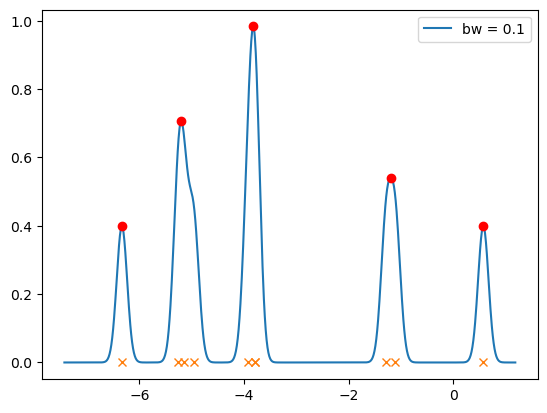
\includegraphics[width=0.27\paperwidth]{pictures/kernel_estim_over.png}
    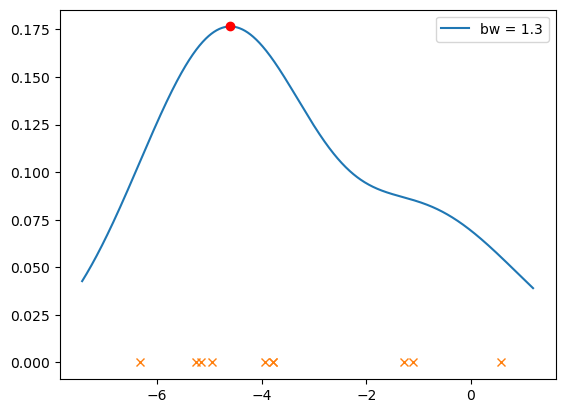
\includegraphics[width=0.27\paperwidth]{pictures/kernel_estim_under.png}
    \caption{(Left): $h$ is to small (Right): $h$ is to large}
    \label{fig:choice_h}
\end{figure}



In his paper , Silverman proves that using a Gaussian kernel ensures that decreasing $h$ will only introduce new local maxima \cite{silverman1981using}. Consequently, it is possible to find the minimum width $h_k$ such that $ \hat f_n(\cdot, h_k)$ has at most $k$ maxima for any integer $k \in \{1, \cdots, n\}$. \\

The estimator $\hat f_n(\cdot, h_k)$ form a family of kernel estimators, each with at most $k$ modes. In his paper, Silverman proposes a procedure for determining the significance of each of them. 

To do this, he uses a bootstrap method. The principle consists to evaluate the accuracy of the estimator by computing it on observations that are resampled from the original set of observations. \\

\textit{Methodology to evaluate the accuracy of the estimator} $\hat f(\cdot, h_k)$
\begin{enumerate}
    \item  First, draw a $n$-sample $X_{I(i)}$ with replacement from the the original set of observations
    \item Add some noise
    \begin{align*}
        y_i = \frac{1}{1+h_k^2/\sigma^2}(X_I(i) + h_k \varepsilon_i)
    \end{align*}
    where $\sigma$ is the standard deviation of $X_1, \ldots, X_n$, $h_k$ is the critical width we are testing, and $\varepsilon_i$ is a random value sampled from a normal distribution with mean 0 and standard deviation 1.
    \item Compute $\hat f_n(\cdot, h_k)$ for sample $y_i$. Check if $\hat f_n(\cdot, h_k)$ has less than $k$--mode. 
    \item Repeat. By repeating this operation several times, we calculate the $p$-value as the fraction of simulations where we did not find more than k modes.
\end{enumerate}


\subsubsection{Numerical examples}

\paragraph{A Gaussian mixture with 2 modes.} We illustrate the Silverman's test on the Gaussian mixture $0.6\mathcal{N}(-5,1)+0.4\mathcal{N}(0,1)$.
\begin{table}
\centering
\begin{tabular}{c|c|l}
Null hypothesis & p--value & bandwitdh \\
\hline
Reject 1 mode & p-value 0.99  & $h_1$ \, 1.3595962524414062 \\
Reject 2 mode & p-value 0.48  & $h_2$ \, 0.35981178283691406 \\
Reject 3 mode & p-value 0.75  & $h_3$ \, 0.33596038818359375 \\
Reject 4 mode & p-value 0.45  & $h_4$ \, 0.24213790893554688 \\
\end{tabular}
\caption{Result of the Silverman test for the Gaussian mixture with 2 modes}
\label{tab:silver_gm_2mod}
\end{table}
In Tab~\ref{tab:silver_gm_2mod}, we see that the null hypothesis : \textit{The density is unimodal} can be rejected with a $p$--value of 0.99. 

\subsection{The DIP test}

The DIP test, also known as the Hartigan's Dip Test, is a statistical test used to assess the unimodality of a data distribution. It measures the departure of the empirical distribution function of a sample from a unimodal distribution. Specifically, the test computes the maximum difference (or "dip") between the empirical distribution and the best-fitting unimodal distribution (defined as the least convex majorant and greatest convex minorant of the empirical distribution). A significant dip value indicates that the sample is not unimodal, suggesting the presence of multiple modes.

A unimodal distribution will have a Probability Density Function (PDF) that increases from 0 to some peak value and then decrease back to 0. When the PDF reaches a local maximum, then the Cumulative Distribution Function (CDF) switches from convex to concave.
A multimodal distributions CDF will change from convex to concave several times.\\

The concept behind the dip statistic is to gauge the extent of adjustment required for the cumulative distribution function (CDF) to become unimodal. Specifically, it represents the greatest distance, observed at any point, between the CDF and the nearest multimodal CDF. To put it differently, we can transform the distribution into a unimodal form by shifting the CDF by no more than the dip value at each instance. Essentially, the dip corresponds to the minimum value needed to achieve this transformation throughout the distribution.



\subsection{The Excess mass test}

\subsubsection{Presentation of the test}
The Excess Mass test is a statistical method used to assess multimodality in a data distribution by comparing the amount of probability mass concentrated in potential modes to what would be expected under unimodality.  It has been introduced by Müller and Sawitzki in 1991 \cite{muller1991excess}. The test evaluates the presence of multiple peaks by measuring the "excess mass," which refers to the extra density that appears around modes beyond what would be expected if the distribution were unimodal.

The Excess Mass test works by identifying regions in the data with significant density peaks and then calculating the total probability mass within these regions. This excess mass is compared to a reference unimodal distribution through optimization, which seeks to maximize the difference between observed density peaks and the unimodal fit. A significant excess mass indicates that the distribution has more than one mode.

The test is flexible and can be adjusted for different modes' widths and shapes, making it suitable for detecting multimodality in complex or irregular distributions. It is particularly useful in settings where traditional methods, like kernel density estimation, might struggle to identify multimodal structures. The results are typically interpreted through p-values or other statistical measures derived from comparisons with reference distributions generated via simulation or other means.\\


The empirical excess mass for $k$ modes and a constant $\lambda$ is defined as
\begin{align*}
    E_{n,k}(\PP, \lambda) = \sup_{C_1(\lambda), \ldots, C_k(\lambda)}
    \left\{
    \sum_{m = 1}^k \PP_n(C_m(\lambda))-\lambda\| C_m(\lambda)\|
    \right\}
\end{align*}
where the supremum is taken over all families $\{ C_m(\lambda) : m = 1, \ldots, l\}$ of closed intervals with endpoints at data points. $\|C_m\|$ denotes the measure of $C_m(\lambda)$ and 
\begin{align*}
    \PP_n(C_m(\lambda)) 
    = \frac{1}{n}\sum_{i = 1}^n
    \mathbb{1}_{X_i \in C_m(\lambda)}
\end{align*}

The key idea is that the difference $D_{n, k+1}(\lambda) = E_{n,k+1}(\PP, \lambda) - E_{n,k}(\PP, \lambda)$ represents the plausibility of the null hypothesis. The larger $D_{n, k+1}(\lambda)$ is, the more likely we are to reject $H_0$. \\

The excess mass statistic is defined as 
\begin{align*}
    \Delta_{n, k+1} = \max_{\lambda}\{D_{n, k+1}(\lambda)\}
\end{align*}

\subsubsection{Numerical examples}

\section{An application to the biological problem}
In this section, we apply 
\label{s:multimod_application}
\subsection{Simulation without noise}
\subsection{Simulation with noise}
\subsection{Real dataset}